\ifx\wholebook\relax \else
% ------------------------

\documentclass[UTF8]{article}
%------------------- Other types of document example ------------------------
%
%\documentclass[twocolumn]{IEEEtran-new}
%\documentclass[12pt,twoside,draft]{IEEEtran}
%\documentstyle[9pt,twocolumn,technote,twoside]{IEEEtran}
%
%-----------------------------------------------------------------------------
%
% loading packages
%

\RequirePackage{ifpdf}
\RequirePackage{ifxetex}

%
%
\ifpdf
  \RequirePackage[pdftex,%
       bookmarksnumbered,%
              colorlinks,%
          linkcolor=blue,%
              hyperindex,%
        plainpages=false,%
       pdfstartview=FitH]{hyperref}
\else\ifxetex
  \RequirePackage[bookmarksnumbered,%
               colorlinks,%
           linkcolor=blue,%
               hyperindex,%
         plainpages=false,%
        pdfstartview=FitH]{hyperref}
\else
  \RequirePackage[dvipdfm,%
        bookmarksnumbered,%
               colorlinks,%
           linkcolor=blue,%
               hyperindex,%
         plainpages=false,%
        pdfstartview=FitH]{hyperref}
\fi\fi
%\usepackage{hyperref}

% other packages
%--------------------------------------------------------------------------
\usepackage{graphicx, color}
\usepackage{subfig}
\usepackage{tikz}
\usetikzlibrary{matrix,positioning}

\usepackage{amsmath, amsthm, amssymb} % for math
\usepackage{exercise} % for exercise
\usepackage{import} % for nested input

%
% for programming
%
\usepackage{verbatim}
\usepackage{listings}
%\usepackage{algorithmic} %old version; we can use algorithmicx instead
\usepackage{algorithm}
\usepackage[noend]{algpseudocode} %for pseudo code, include algorithmicsx automatically
\usepackage{appendix}
\usepackage{makeidx} % for index support
\usepackage{titlesec}

\usepackage[cm-default]{fontspec}
\usepackage{xunicode}

% detect and select Chinese font
% ------------------------------
% the following cmd can list all availabe Chinese fonts in host.
% fc-list :lang=zh
\def\myfont{STHeiti}  % Under Mac OS X
\def\linuxfallback{WenQuanYi Micro Hei} % Under Linux
\def\winfallback{SimSun} % Under Windows
\suppressfontnotfounderror1 % Avoid setting exit code (error level) to break make process
\count255=\interactionmode
\batchmode
\font\foo="\myfont"\space at 10pt
\ifx\foo\nullfont
  \font\foo = "\linuxfallback"\space at 10pt
  \ifx\foo\nullfont
    \font\foo = "\winfallback"\space at 10pt
    \ifx\foo\nullfont
      \errorstopmode
      \errmessage{no suitable Chinese font found}
    \else
      \let\myfont=\winfallback % Windows
    \fi
  \else
    \let\myfont=\linuxfallback % Linux
  \fi
\fi
\interactionmode=\count255
\setmainfont[Mapping=tex-text]{\myfont}

\XeTeXlinebreaklocale "zh"  % to solve the line breaking issue
\XeTeXlinebreakskip = 0pt plus 1pt minus 0.1pt

\titleformat{\paragraph}
{\normalfont\normalsize\bfseries}{\theparagraph}{1em}{}
\titlespacing*{\paragraph}
{0pt}{3.25ex plus 1ex minus .2ex}{1.5ex plus .2ex}

\lstdefinelanguage{Smalltalk}{
  morekeywords={self,super,true,false,nil,thisContext}, % This is overkill
  morestring=[d]',
  morecomment=[s]{"}{"},
  alsoletter={\#:},
  escapechar={!},
  literate=
    {BANG}{!}1
    {UNDERSCORE}{\_}1
    {\\st}{Smalltalk}9 % convenience -- in case \st occurs in code
    % {'}{{\textquotesingle}}1 % replaced by upquote=true in \lstset
    {_}{{$\leftarrow$}}1
    {>>>}{{\sep}}1
    {^}{{$\uparrow$}}1
    {~}{{$\sim$}}1
    {-}{{\sf -\hspace{-0.13em}-}}1  % the goal is to make - the same width as +
    %{+}{\raisebox{0.08ex}{+}}1		% and to raise + off the baseline to match -
    {-->}{{\quad$\longrightarrow$\quad}}3
	, % Don't forget the comma at the end!
  tabsize=2
}[keywords,comments,strings]

% for better Haskell code outlook
\lstdefinelanguage{Haskell}{
  basicstyle=\small\ttfamily,
  flexiblecolumns=false,
  basewidth={0.5em,0.45em},
  literate={+}{{$+$}}1 {/}{{$/$}}1 {*}{{$*$}}1 {=}{{$=$}}1
           {>}{{$>$}}1 {<}{{$<$}}1 {\\}{{$\lambda$}}1
           {\\\\}{{\char`\\\char`\\}}1
           {->}{{$\rightarrow$}}2 {>=}{{$\geq$}}2 {<-}{{$\leftarrow$}}2
           {<=}{{$\leq$}}2 {=>}{{$\Rightarrow$}}2
           {\ .}{{$\circ$}}2 {\ .\ }{{$\circ$}}2
           {>>}{{>>}}2 {>>=}{{>>=}}2
           {|}{{$\mid$}}1
}[keywords,comments,strings]

\lstloadlanguages{C, C++, Lisp, Haskell, Python, Smalltalk}

\lstset{
  showstringspaces = false
}

% ======================================================================

\def\BibTeX{{\rm B\kern-.05em{\sc i\kern-.025em b}\kern-.08em
    T\kern-.1667em\lower.7ex\hbox{E}\kern-.125emX}}

%
% mathematics
%
\newcommand{\be}{\begin{equation}}
\newcommand{\ee}{\end{equation}}
\newcommand{\bmat}[1]{\left( \begin{array}{#1} }
\newcommand{\emat}{\end{array} \right) }
\newcommand{\VEC}[1]{\mbox{\boldmath $#1$}}

% numbered equation array
\newcommand{\bea}{\begin{eqnarray}}
\newcommand{\eea}{\end{eqnarray}}

% equation array not numbered
\newcommand{\bean}{\begin{eqnarray*}}
\newcommand{\eean}{\end{eqnarray*}}

\newtheorem{theorem}{Theorem}[section]
\newtheorem{lemma}[theorem]{Lemma}
\newtheorem{proposition}[theorem]{Proposition}
\newtheorem{corollary}[theorem]{Corollary}


\setcounter{page}{1}

\begin{document}

%--------------------------

% ================================================================
%                 COVER PAGE
% ================================================================

\title{从吃葡萄到世界杯,选择排序的进化}

\author{刘新宇
\thanks{{\bfseries 刘新宇 } \newline
  Email: liuxinyu95@gmail.com \newline}
  }

\maketitle
\fi

\markboth{选择排序}{初等算法}

\ifx\wholebook\relax
\chapter{从吃葡萄到世界杯,选择排序的进化}
\numberwithin{Exercise}{chapter}
\fi

% ================================================================
%                 Introduction
% ================================================================
\section{简介}
\label{introduction} \index{选择排序}

我们此前介绍了排序中的“hello world”―插入排序算法。本章中,我们介绍另外一种直观的排序方法―选择排序。最基本的选择排序在性能上不如分而治之排序算法,如快速排序和归并排序。同插入排序那一章一样,我们将会分析为什么选择排序的速度慢,并且从不同的角度改进它,最终进化到堆排序,从而达到基于比较的排序的性能上限$O(n \lg n)$。

选择排序的思想在日常生活中很常见。考虑一个小孩要吃掉一串葡萄。我们通常会发现两种类型的小孩,一种属于“乐观型”,每次吃掉最大的一颗;另一种属于“悲观型”,每次总吃掉最小的一颗。

第一种小孩实际上按照由大到小的顺序吃葡萄;第二种按照由小到大的顺序吃葡萄。实际上,孩子把葡萄按照大小进行了\underline{排序},并且使用了选择排序的方法。
\begin{figure}[htbp]
  \centering
  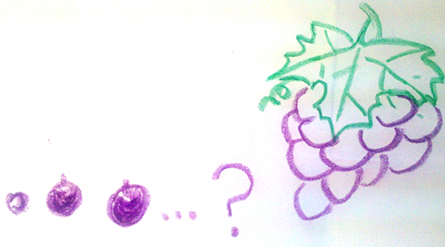
\includegraphics[scale=0.6]{img/grapes-1.eps}
  \caption{总挑出最小的葡萄。}
  \label{fig:eat-grapes}
\end{figure}

Based on this idea, the algorithm of selection sort can be directly
described as the following.

In order to sort a series of elements:

\begin{itemize}
\item The trivial case, if the series is empty, then we are done, the result is also empty;
\item Otherwise, we find the smallest element, and append it to the tail of the result;
\end{itemize}

Note that this algorithm sorts the elements in increase order; It's easy to sort in decrease
order by picking the biggest element instead; We'll introduce about passing a comparator as
a parameter later on.

This description can be formalized to a equation.

\be
sort(A) =  \left \{
  \begin{array}
  {r@{\quad:\quad}l}
  \phi & A = \phi \\
  \{ m \} \cup sort(A') & otherwise
  \end{array}
\right.
\ee

Where $m$ is the minimum element among collection $A$, and $A'$ is all the rest elements
except $m$:

\[
\begin{array}{l}
m = min(A) \\
A' = A - \{ m \}
\end{array}
\]

We don't limit the data structure of the collection here. Typically, $A$ is an array in imperative
environment, and a list (singly linked-list particularly) in functional environment, and it can even
be other data struture which will be introduced later.

The algorithm can also be given in imperative manner.

\begin{algorithmic}
\Function{Sort}{$A$}
  \State $X \gets \phi$
  \While{$A \neq \phi$}
    \State $x \gets$ \Call{Min}{$A$}
    \State $A \gets$ \Call{Del}{$A, x$}
    \State $X \gets$ \Call{Append}{$X, x$}
  \EndWhile
  \State \Return $X$
\EndFunction
\end{algorithmic}

Figure \ref{fig:sel-sort} depicts the process of this algorithm.

\begin{figure}[htbp]
  \centering
  \includegraphics[scale=0.8]{img/sel-sort.ps}
  \caption{The left part is sorted data, continuously pick the minimum element in the rest and append it to the result.}
  \label{fig:sel-sort}
\end{figure}

We just translate the very original idea of `eating grapes' line by line without
considering any expense of time and space. This realization stores the result
in $X$, and when an selected element is appended to $X$, we delete the same element
from $A$. This indicates that we can change it to `in-place' sorting to reuse
the spaces in $A$.

The idea is to store the minimum element in the first cell in $A$ (we use term `cell' if
$A$ is an array, and say `node' if $A$ is a list); then store the second minimum element
in the next cell, then the third cell, ...

One solution to realize this sorting strategy is swapping. When we select the $i$-th
minimum element, we swap it with the element in the $i$-th cell:

\begin{algorithmic}
\Function{Sort}{$A$}
  \For{$i \gets 1$ to $|A|$}
    \State $m \gets$ \Call{Min}{$A[i...]$}
    \State \textproc{Exchange} $A[i] \leftrightarrow m$
  \EndFor
\EndFunction
\end{algorithmic}

Denote $A = \{a_1, a_2, ..., a_N\}$. At any time, when we process the $i$-th element,
all elements before $i$, as $\{a_1, a_2, ..., a_{i-1}\}$ have already been sorted.
We locate the minimum element among the $\{a_i, a_{i+1}, ..., a_N\}$, and exchange it
with $a_i$, so that the $i$-th cell contains the right value. The process is repeatedly
executed until we arrived at the last element.

This idea can be illustrated by figure \ref{fig:in-place-sort}.

\begin{figure}[htbp]
  \centering
  \includegraphics[scale=0.8]{img/in-place-sort.ps}
  \caption{The left part is sorted data, continuously pick the minimum element in the rest and put it to the right position.}
  \label{fig:in-place-sort}
\end{figure}

% ================================================================
% Find the minimum
% ================================================================
\section{Finding the minimum}
\index{selection sort!minimum finding}

We haven't completely realized the selection sort, because we take the operation
of finding the minimum (or the maximum) element as a black box. It's a puzzle how does
a kid locate the biggest or the smallest grape.
And this is an interesting topic for computer algorithms.

The easiest but not so fast way to find the minimum in a collection is to perform
a scan. There are several ways to interpret this scan process. Consider that
we want to pick the biggest grape. We start from any grape, compare it with
another one, and pick the bigger one; then we take a next grape and compare
it with the one we selected so far, pick the bigger one and go on the take-and-compare
process, until there are not any grapes we haven't compared.

It's easy to get loss in real practice if we don't mark which grape has been
compared. There are two ways to to solve this problem, which are suitable for
different data-structures respectively.

\subsection{Labeling}
Method 1 is to label each grape with a number: $\{1, 2, ..., N\}$, and we systematically
perform the comparison in the order of this sequence of labels. That we first
compare grape number 1 and grape number 2, pick the bigger one; then we take grape
number 3, and do the comparison, ... We repeat this process until arrive at
grape number $N$. This is quite suitable for elements stored in an array.

\begin{algorithmic}
\Function{Min}{$A$}
  \State $m \gets A[1]$
  \For{$i \gets 2$ to $|A|$}
    \If{$A[i] < m$}
      \State $m \gets A[i]$
    \EndIf
  \EndFor
  \State \Return $m$
\EndFunction
\end{algorithmic}

With \textproc{Min} defined, we can complete the basic version of selection sort
(or naive version without any optimization in terms of time and space).

However, this algorithm returns the value of the minimum element instead of its
location (or the label of the grape), which needs a bit tweaking for the in-place version.
Some languages such as ISO C++, support returning the reference as result, so that the
swap can be achieved directly as below.

\lstset{language=C++}
\begin{lstlisting}
template<typename T>
T& min(T* from, T* to) {
    T* m;
    for (m = from++; from != to; ++from)
        if (*from < *m)
            m = from;
    return *m;
}

template<typename T>
void ssort(T* xs, int n) {
    int i;
    for (i = 0; i < n; ++i)
        std::swap(xs[i], min(xs+i, xs+n));
}
\end{lstlisting}

In environments without reference semantics, the solution is to return the location
of the minimum element instead of the value:

\begin{algorithmic}
\Function{Min-At}{$A$}
  \State $m \gets$ \Call{First-Index}{$A$}
  \For{$i \gets m + 1 $ to $|A|$}
    \If{$A[i] < A[m]$}
      \State $m \gets i$
    \EndIf
  \EndFor
  \State \Return $m$
\EndFunction
\end{algorithmic}

Note that since we pass $A[i...]$ to \textproc{Min-At} as the argument, we assume the first
element $A[i]$ as the smallest one, and examine all elements $A[i+1], A[i+2], ...$ one by one.
Function \textproc{First-Index}() is used to retrieve $i$ from the input parameter.

The following Python example program, for example, completes the basic in-place
selection sort algorithm based on this idea. It explicitly passes the range information
to the function of finding the minimum location.

\lstset{language=Python}
\begin{lstlisting}
def ssort(xs):
    n = len(xs)
    for i in range(n):
        m = min_at(xs, i, n)
        (xs[i], xs[m]) = (xs[m], xs[i])
    return xs

def min_at(xs, i, n):
    m = i;
    for j in range(i+1, n):
        if xs[j] < xs[m]:
            m = j
    return m
\end{lstlisting}

\subsection{Grouping}
\index{selection sort!tail-recursive call minimum finding}
Another method is to group all grapes in two parts: the group we have examined, and the rest we
haven't. We denote these two groups as $A$ and $B$; All the elements (grapes) as $L$.
At the beginning, we haven't examine any grapes at all, thus $A$ is empty ($\phi$), and
$B$ contains all grapes. We can select arbitrary two grapes from $B$, compare them, and
put the loser (the smaller one for example) to $A$. After that, we repeat this process
by continuously picking arbitrary grapes from $B$, and compare with the winner of the
previous time until $B$ becomes empty. At this time being, the final winner is the
minimum element. And $A$ turns to be $L - \{min(L)\}$, which can be used for the next
time minimum finding.

There is an invariant of this method, that at any time, we have $L = A \cup \{m\} \cup B$,
where $m$ is the winner so far we hold.

This approach doesn't need the collection of grapes being indexed (as being labeled
in method 1). It's suitable for any traversable data structures, including linked-list
etc. Suppose $b_1$ is an arbitrary element in $B$ if $B$ isn't empty, and $B'$ is
the rest of elements with $b_1$ being removed,
this method can be formalized as the below auxiliary function.

\be
min'(A, m, B) =  \left \{
  \begin{array}
  {r@{\quad:\quad}l}
  (m, A) & B = \phi \\
  min'(A \cup \{m\}, b_1, B') & b_1 < m \\
  min'(A \cup \{b_1\}, m, B') & otherwise
  \end{array}
\right.
\ee

In order to pick the minimum element, we call this auxiliary function by passing
an empty $A$, and use an arbitrary element (for instance, the first one)
to initialize $m$:

\be
extractMin(L) = min'(\phi, l_1, L')
\ee

Where $L'$ is all elements in $L$ except for the first one $l_1$. The algorithm
$extractMin)$ doesn't not only find the minimum element, but also returns the
updated collection which doesn't contain this minimum. Summarize this minimum
extracting algorithm up to the basic selection sort definition, we can create
a complete functional sorting program, for example as this Haskell code snippet.

\lstset{language=Haskell}
\begin{lstlisting}
sort [] = []
sort xs = x : sort xs' where
  (x, xs') = extractMin xs

extractMin (x:xs) = min' [] x xs where
  min' ys m [] = (m, ys)
  min' ys m (x:xs) = if m < x then min' (x:ys) m xs else min' (m:ys) x xs
\end{lstlisting}

The first line handles the trivial edge case that the sorting result for empty
list is obvious empty; The second clause ensures that, there is at least one
element, that's why the \verb|extractMin| function needn't other pattern-matching.

One may think the second clause of \verb|min'| function should be written like below:

\begin{lstlisting}
min' ys m (x:xs) = if m < x then min' ys ++ [x] m xs
                            else min' ys ++ [m] x xs
\end{lstlisting}

Or it will produce the updated list in reverse order. Actually, it's necessary to
use `cons' instead of appending here. This is because appending is linear operation
which is proportion to the length of part $A$, while `cons' is constant $O(1)$ time
operation. In fact, we needn't keep the relative order of the list to be sorted,
as it will be re-arranged anyway during sorting.

It's quite possible to keep the relative order during sorting, while ensure the
performance of finding the minimum element not degrade to quadratic. The following
equation defines a solution.

\be
extractMin(L) = \left \{
  \begin{array}
  {r@{\quad:\quad}l}
  (l_1, \phi) & |L| = 1 \\
  (l_1, L') & l_1 < m, (m, L'') = extractMin(L') \\
  (m, {l_1} \cup L'') & otherwise
  \end{array}
\right.
\ee

If $L$ is a singleton, the minimum is the only element it contains. Otherwise,
denote $l_1$ as the first element in $L$, and $L'$ contains the rest elements except
for $l_1$, that $L' = \{ l_2, l_3, ...\}$. The algorithm recursively finding
the minimum element in $L'$, which yields the intermediate result as $(m, L'')$,
that $m$ is the minimum element in $L'$, and $L''$ contains all rest elements
except for $m$. Comparing $l_1$ with $m$, we can determine which of them is
the final minimum result.

The following Haskell program implements this version of selection sort.

\begin{lstlisting}
sort [] = []
sort xs = x : sort xs' where
  (x, xs') = extractMin xs

extractMin [x] = (x, [])
extractMin (x:xs) = if x < m then (x, xs) else (m, x:xs') where
  (m, xs') = extractMin xs
\end{lstlisting}

Note that only `cons' operation is used, we needn't appending at all because
the algorithm actually examines the list from right to left. However, it's not
free, as this program need book-keeping the context (via call stack typically).
The relative order is ensured by the nature of recursion. Please refer
to the appendix about tail recursion call for detailed discussion.

\subsection{performance of the basic selection sorting}

Both the labeling method, and the grouping method need examine all the elements to
pick the minimum in every round; and we totally pick up the minimum element $n$ times.
Thus the performance is around $n + (n-1) + (n-2) + ... + 1$ which is $\frac{n(n+1)}{2}$.
Selection sort is a quadratic algorithm bound to $O(n^2)$ time.

Compare to the insertion sort, which we introduced previously, selection sort
performs same in its best case, worst case and average case. While insertion
sort performs well in best case (that the list has been reverse ordered, and it is stored
in linked-list) as $O(n)$, and the worst performance is $O(n^2)$.

In the next sections, we'll examine, why selection sort performs poor, and try
to improve it step by step.

\begin{Exercise}

\begin{itemize}
\item Implement the basic imperative selection sort algorithm (the none in-place version)
in your favorite programming language. Compare it with the in-place version, and analyze
the time and space effectiveness.
\end{itemize}

\end{Exercise}

% ================================================================
% Improvement 1
% ================================================================

\section{Minor Improvement}

\subsection{Parameterize the comparator}
\index{selection sort!parameterize the comparator}
Before any improvement in terms of performance, let's make the selection sort
algorithm general enough to handle different sorting criteria.

We've seen two opposite examples so far, that one may need sort the elements
in ascending order or descending order. For the former case, we need
repeatedly finding the minimum, while for the later, we need find the maximum
instead. They are just two special cases. In real world practice, one
may want to sort things in varies criteria, e.g. in terms of size, weight,
age, ...

One solution to handle them all is to passing the criteria as a compare function
to the basic selection sort algorithms. For example:

\be
sort(c, L) = \left \{
  \begin{array}
  {r@{\quad:\quad}l}
  \phi & L = \phi \\
  {m} \cup sort(c, L'') & otherwise, (m, L'') = extract(c, L')
  \end{array}
\right.
\ee

And the algorithm $extract(c, L)$ is defined as below.

\be
extract(c, L) = \left \{
  \begin{array}
  {r@{\quad:\quad}l}
  (l_1, \phi) & |L| = 1 \\
  (l_1, L') & c(l_1, m), (m, L'') = extract(c, L') \\
  (m, \{l_1\} \cup L'') & \lnot c(l_1, m)
  \end{array}
\right.
\ee

Where $c$ is a comparator function, it takes two elements, compare them and
returns the result of which one is preceding of the other.
Passing `less than' operator $(<)$ turns this algorithm to be the version
we introduced in previous section.

Some environments require to pass the total ordering comparator, which
returns result among `less than', 'equal', and 'greater than'. We needn't
such strong condition here, that $c$ only tests if `less than' is satisfied.
However, as the minimum requirement, the comparator should meet the
strict weak ordering as following \cite{wiki-sweak-order}:

\begin{itemize}
\item Irreflexivity, for all $x$, it's not the case that $x < x$;
\item Asymmetric, For all $x$ and $y$, if $x < y$, then it's not the case $y < x$;
\item Transitivity, For all $x$, $y$, and $z$, if $x < y$, and $y < z$, then $x < z$;
\end{itemize}

The following Scheme/Lisp program translates this generic selection sorting algorithm.
The reason why we choose Scheme/Lisp here is because the lexical scope can simplify
the needs to pass the `less than' comparator for every function calls.

\lstset{language=Lisp}
\begin{lstlisting}
(define (sel-sort-by ltp? lst)
  (define (ssort lst)
    (if (null? lst)
        lst
        (let ((p (extract-min lst)))
          (cons (car p) (ssort (cdr p))))))
  (define (extract-min lst)
    (if (null? (cdr lst))
        lst
        (let ((p (extract-min (cdr lst))))
          (if (ltp? (car lst) (car p))
              lst
              (cons (car p) (cons (car lst) (cdr p)))))))
  (ssort lst))
\end{lstlisting}

Note that, both \verb|ssort| and \verb|extract-min| are inner functions, so that the
`less than' comparator \verb|ltp?| is available to them. Passing `$<$' to this function
yields the normal sorting in ascending order:

\lstset{language=Lisp}
\begin{lstlisting}
(sel-sort-by < '(3 1 2 4 5 10 9))
;Value 16: (1 2 3 4 5 9 10)
\end{lstlisting}

It's possible to pass varies of comparator to imperative selection sort as well. This
is left as an exercise to the reader.

For the sake of brevity, we only consider sorting elements in ascending order in
the rest of this chapter. And we'll not pass comparator as a parameter unless it's
necessary.

\subsection{Trivial fine tune}

The basic in-place imperative selection sorting algorithm iterates all elements, and picking the
minimum by traversing as well. It can be written in a compact way, that we
inline the minimum finding part as an inner loop.

\begin{algorithmic}
\Procedure{Sort}{$A$}
  \For{ $i \gets 1$ to $|A|$}
    \State $m \gets i$
    \For{$j \gets i+1$ to $|A|$}
      \If{$A[i] < A[m]$}
        \State $m \gets i$
      \EndIf
    \EndFor
    \State \textproc{Exchange} $A[i] \leftrightarrow A[m]$
  \EndFor
\EndProcedure
\end{algorithmic}

Observe that, when we are sorting $N$ elements, after the first $N-1$ minimum ones are selected,
the left only one, is definitely the $N$-th big element, so that we need NOT find the
minimum if there is only one element in the list. This indicates that the outer loop can
iterate to $N-1$ instead of $N$.

Another place we can fine tune, is that we needn't swap the elements if the $i$-th minimum one
is just $A[i]$. The algorithm can be modified accordingly as below:

\begin{algorithmic}
\Procedure{Sort}{$A$}
  \For{ $i \gets 1$ to $|A|-1$}
    \State $m \gets i$
    \For{$j \gets i+1$ to $|A|$}
      \If{$A[i] < A[m]$}
        \State $m \gets i$
      \EndIf
    \EndFor
    \If{$m \neq i$}
      \State \textproc{Exchange} $A[i] \leftrightarrow A[m]$
    \EndIf
  \EndFor
\EndProcedure
\end{algorithmic}

Definitely, these modifications won't affects the performance in terms of big-O.

\subsection{Cock-tail sort}
\index{Cock-tail sort}
Knuth gave an alternative realization of selection sort in \cite{TAOCP}. Instead of selecting the
minimum each time, we can select the maximum element, and put it to the last position. This method
can be illustrated by the following algorithm.

\begin{algorithmic}
\Procedure{Sort'}{$A$}
  \For{ $i \gets |A|$ down-to $2$}
    \State $m \gets i$
    \For{$j \gets 1$ to $i-1$}
      \If{$A[m] < A[i]$}
        \State $m \gets i$
      \EndIf
    \EndFor
    \State \textproc{Exchange} $A[i] \leftrightarrow A[m]$
  \EndFor
\EndProcedure
\end{algorithmic}

As shown in figure \ref{fig:knuth-ssort}, at any time, the elements on right most side
are sorted. The algorithm scans all unsorted ones, and locate the maximum. Then, put
it to the tail of the unsorted range by swapping.

\begin{figure}[htbp]
  \centering
  \includegraphics[scale=0.8]{img/knuth-ssort.ps}
  \caption{Select the maximum every time and put it to the end.}
  \label{fig:knuth-ssort}
\end{figure}

This version reveals the fact that, selecting the maximum element can sort the element in
ascending order as well. What's more, we can find both the minimum and the maximum elements
in one pass of traversing, putting the minimum at the first location, while putting the
maximum at the last position. This approach can speed up the sorting slightly (halve the
times of the outer loop).

\begin{algorithmic}
\Procedure{Sort}{$A$}
  \For{$i \gets 1 $ to $\lfloor \frac{|A|}{2} \rfloor$}
    \State $min \gets i$
    \State $max \gets |A| + 1 - i$
    \If{$A[max] < A[min]$}
      \State \textproc{Exchange} $A[min] \leftrightarrow A[max]$
    \EndIf
    \For{$j \gets i + 1$ to $|A| - i$}
      \If{$A[j] < A[min]$}
        \State $min \gets j$
      \EndIf
      \If{$A[max] < A[j]$}
        \State $max \gets j$
      \EndIf
    \EndFor
    \State \textproc{Exchange} $A[i] \leftrightarrow A[min]$
    \State \textproc{Exchange} $A[|A|+1-i] \leftrightarrow A[max]$
  \EndFor
\EndProcedure
\end{algorithmic}

This algorithm can be illustrated as in figure \ref{fig:cock-tail-sort}, at any time, the left most and right most
parts contain sorted elements so far. That the smaller sorted ones are on the left, while the bigger sorted ones
are on the right. The algorithm scans the unsorted ranges, located both the minimum and the maximum positions,
then put them to the head and the tail position of the unsorted ranges by swapping.

\begin{figure}[htbp]
  \centering
  \includegraphics[scale=0.7]{img/cock-tail-sort.ps}
  \caption{Select both the minimum and maximum in one pass, and put them to the proper positions.}
  \label{fig:cock-tail-sort}
\end{figure}

Note that it's necessary to swap the left most and right most elements before the inner loop if they are
not in correct order. This is because we scan the range excluding these two elements. Another method is to
initialize the first element of the unsorted range as both the maximum and minimum before the inner loop.
However, since we need two swapping operations after the scan, it's possible that the first swapping moves
the maximum or the minimum from the position we just found, which leads the second swapping malfunctioned.
How to solve this problem is left as exercise to the reader.

The following Python example program implements this cock-tail sort algorithm.

\lstset{language=Python}
\begin{lstlisting}
def cocktail_sort(xs):
    n = len(xs)
    for i in range(n / 2):
        (mi, ma) = (i, n - 1 -i)
        if xs[ma] < xs[mi]:
            (xs[mi], xs[ma]) = (xs[ma], xs[mi])
        for j in range(i+1, n - 1 - i):
            if xs[j] < xs[mi]:
                mi = j
            if xs[ma] < xs[j]:
                ma = j
        (xs[i], xs[mi]) = (xs[mi], xs[i])
        (xs[n - 1 - i], xs[ma]) = (xs[ma], xs[n - 1 - i])
    return xs
\end{lstlisting}

It's possible to realize cock-tail sort in functional approach as well. An intuitive recursive description
can be given like this:

\begin{itemize}
  \item Trivial edge case: If the list is empty, or there is only one element in the list, the sorted result is obviously the origin list;
  \item Otherwise, we select the minimum and the maximum, put them in the head and tail positions, then recursively sort the rest elements.
\end{itemize}

This algorithm description can be formalized by the following equation.

\be
sort(L) = \left \{
  \begin{array}
  {r@{\quad:\quad}l}
  L & |L| \leq 1 \\
  \{ l_{min} \} \cup sort(L'') \cup \{ l_{max} \} & otherwise
  \end{array}
\right.
\ee

Where the minimum and the maximum are extracted from $L$ by a function $select(L)$.

\[
(l_{min}, L'', l_{max}) = select(L)
\]

Note that, the minimum is actually linked to the front of the recursive sort result. Its semantic is a constant $O(1)$
time `cons' (refer to the appendix of this book for detail). While the maximum is appending to the tail. This
is typically a linear $O(n)$ time expensive operation. We'll optimize it later.

Function $select(L)$ scans the whole list to find both the minimum and the maximum. It can be defined as below:

\be
select(L) =  \left \{
  \begin{array}
  {r@{\quad:\quad}l}
  (min(l_1, l_2), max(l_1, l_2)) & L = \{ l_1, l_2\} \\
  (l_1, \{ l_{min}\} \cup L'', l_{max}) & l_1 < l_{min} \\
  (l_{min}, \{l_{max}\} \cup L'', l_1) & l_{max} < l_1 \\
  (l_{min}, \{l_1\} \cup L'', l_{max}) & otherwise
  \end{array}
\right.
\ee

Where $(l_{min}, L'', l_{max}) = select(L')$ and $L'$ is the rest of the list except for the first element $l_1$.
If there are only two elements in the list, we pick the smaller as the minimum, and the bigger as the maximum.
After extract them, the list becomes empty. This is the trivial edge case; Otherwise, we take the first element
$l_1$ out, then recursively perform selection on the rest of the list. After that, we compare if $l_1$ is less
then the minimum or greater than the maximum candidates, so that we can finalize the result.

Note that for all the cases, there is no appending operation to form the result. However, since selection must
scan all the element to determine the minimum and the maximum, it is bound to $O(n)$ linear time.

The complete example Haskell program is given as the following.

\lstset{language=Haskell}
\begin{lstlisting}
csort [] = []
csort [x] = [x]
csort xs = mi : csort xs' ++ [ma] where
  (mi, xs', ma) = extractMinMax xs

extractMinMax [x, y] = (min x y, [], max x y)
extractMinMax (x:xs) | x < mi = (x, mi:xs', ma)
                     | ma < x = (mi, ma:xs', x)
                     | otherwise = (mi, x:xs', ma)
  where (mi, xs', ma) = extractMinMax xs
\end{lstlisting}

We mentioned that the appending operation is expensive in this intuitive version. It can be improved.
This can be achieved in two steps. The first step is to convert the cock-tail sort into tail-recursive
call. Denote the sorted small ones as $A$, and sorted big ones as $B$ in figure \ref{fig:cock-tail-sort}.
We use $A$ and $B$ as accumulators. The new cock-tail sort is defined as the following.

\be
sort'(A, L, B) = \left \{
  \begin{array}
  {r@{\quad:\quad}l}
  A \cup L \cup B & L = \phi \lor |L| = 1 \\
  sort'(A \cup \{ l_{min}\}, L'', \{ l_{max}\} \cup B) & otherwise
  \end{array}
\right.
\ee

Where $l_{min}$, $l_{max}$ and $L''$ are defined as same as before. And we start sorting by passing
empty $A$ and $B$: $sort(L) = sort'(\phi, L, \phi)$.

Besides the edge case, observing that the appending operation only happens on $A \cup \{l_{min} \}$; while
$l_{max}$ is only linked to the head of $B$. This appending occurs in every recursive call. To eliminate
it, we can store $A$ in reverse order as $\overleftarrow{A}$, so that $l_{max}$ can be `cons' to the
head instead of appending. Denote $cons(x, L) = \{x\} \cup L$ and $append(L, x) = L \cup \{x\}$,
we have the below equation.

\be
\begin{array}{rl}
append(L, x) & = reverse(cons(x, reverse(L))) \\
             & = reverse(cons(x, \overleftarrow{L}))
\end{array}
\ee

Finally, we perform a reverse to turn $\overleftarrow{A}$ back to $A$.
Based on this idea, the algorithm can be improved one more step as the following.

\be
sort'(A, L, B) = \left \{
  \begin{array}
  {r@{\quad:\quad}l}
  reverse(A) \cup B & L = \phi \\
  reverse(\{l_1\} \cup A) \cup B & |L| = 1 \\
  sort'(\{l_{min}\} \cup A, L'', \{l_{max}\} \cup B)
  \end{array}
\right.
\ee

This algorithm can be implemented by Haskell as below.

\lstset{language=Haskell}
\begin{lstlisting}
csort' xs = cocktail [] xs [] where
  cocktail as [] bs = reverse as ++ bs
  cocktail as [x] bs = reverse (x:as) ++ bs
  cocktail as xs bs = let (mi, xs', ma) = extractMinMax xs
                      in cocktail (mi:as) xs' (ma:bs)
\end{lstlisting}

\begin{Exercise}
  \begin{itemize}
    \item Realize the imperative basic selection sort algorithm, which can take a comparator as a parameter. Please try both dynamic typed language and static typed language. How to annotate the type of the comparator as general as possible in a static typed language?
   \item Implement Knuth's version of selection sort in your favorite programming language.
   \item An alternative to realize cock-tail sort is to assume the $i$-th element both the minimum and the maximum, after the inner loop, the minimum and maximum are found, then we can swap the the minimum to the $i$-th position, and
the maximum to position $|A|+1-i$. Implement this solution in your favorite imperative language. Please note that
there are several special edge cases should be handled correctly:
    \begin{itemize}
      \item $A = \{max, min, ...\}$;
      \item $A = \{..., max, min\}$;
      \item $A = \{max, ..., min\}$.
    \end{itemize}
    Please don't refer to the example source code along with this chapter before you try to solve this problem.
  \end{itemize}
\end{Exercise}

% ================================================================
% Improvement 2
% ================================================================

\section{Major improvement}

Although cock-tail sort halves the numbers of loop, the performance is still bound to quadratic time.
It means that, the method we developed so far handles big data poorly compare to other divide and conquer
sorting solutions.

To improve selection based sort essentially, we must analyze where is the bottle-neck. In order to sort
the elements by comparison, we must examine all the elements for ordering. Thus the outer loop of selection
sort is necessary. However, must it scan all the elements every time to select the minimum? Note that
when we pick the smallest one at the first time, we actually traverse the whole collection, so that
we know which ones are relative big, and which ones are relative small partially.

The problem is that, when we select the further minimum elements, instead of re-using the ordering information
we obtained previously, we drop them all, and blindly start a new traverse.

So the key point to improve selection based sort is to re-use the previous result. There are several approaches,
we'll adopt an intuitive idea inspired by football match in this chapter.

\subsection{Tournament knock out}
\index{Trounament knock out}
The football world cup is held every four years. There are 32 teams from different continent
play the final games. Before 1982, there were 16 teams compete for the tournament finals\cite{wiki-wc}.

For simplification purpose, let's go back to 1978 and imagine a way to determine the champion:
In the first round, the teams
are grouped into 8 pairs to play the game; After that, there will be 8 winner, and 8 teams will
be out. Then in the second round, these 8 teams are grouped into 4 pairs. This time there
will be 4 winners after the second round of games; Then the top 4 teams are divided into
2 pairs, so that there will be only two teams left for the final game.

The champion is determined after the total 4 rounds of games. And there are actually $8+4+2+1 = 16$
games. Now we have the world cup champion, however, the world cup game won't finish at this stage,
we need to determine which is the silver medal team.

Readers may argue that isn't the team beaten by the champion at the final game the second best?
This is true according to the real world cup rule. However, it isn't fair enough in some sense.

We often heard about the so called `group of death', Let's suppose that Brazil team is
grouped with Deutch team at the very beginning. Although both teams are quite strong, one of
them must be knocked out. It's quite possible that even the team loss that game can beat
all the other teams except for the champion. Figure \ref{fig:tournament-tree-1} illustrates such
case.

\begin{figure}[htbp]
  \centering
  \includegraphics[scale=0.25]{img/tournament-tree-1.ps}
  \caption{The element 15 is knocked out in the first round.}
  \label{fig:tournament-tree-1}
\end{figure}

Imagine that every team has a number. The bigger the number, the stronger the team. Suppose
that the stronger team always beats the team with smaller number, although this is not true
in real world. But this simplification is fair enough for us to develop the tournament knock
out solution. This maximum number which represents the champion is 16. Definitely, team with
number 14 isn't the second best according to our rules. It should be 15, which is knocked
out at the first round of comparison.

The key question here is to find an effective way to locate the second maximum number in this
tournament tree. After that, what we need is to apply the same method to select the third,
the fourth, ..., to accomplish the selection based sort.

One idea is to assign the champion a very small number (for instance, $-\infty$),
so that it won't be selected next time, and the second best one, becomes the new champion.
However, suppose there are $2^m$ teams for some natural number $m$, it still takes
$2^{m-1} + 2^{m-2} + ... + 2 + 1 = 2^m$ times of comparison to determine the new
champion. Which is as slow as the first time.

Actually, we needn't perform a bottom-up comparison at all since the tournament tree
stores plenty of ordering information. Observe that, the second best team must
be beaten by the champion at sometime, or it will be the final winner. So we
can track the path from the root of the tournament tree to the leaf of the
champion, examine all the teams along with this path to find the second best team.

In figure \ref{fig:tournament-tree-1}, this path is marked in gray color, the elements
to be examined are $\{14, 13, 7, 15\}$. Based on this idea, we refine the algorithm
like below.

\begin{enumerate}
\item Build a tournament tree from the elements to be sorted, so that the champion (the maximum) becomes the root;
\item Extract the root from the tree, perform a top-down pass and replace the maximum with $-\infty$;
\item Perform a bottom-up back-track along the path, determine the new champion and make it as the new root;
\item Repeat step 2 until all elements have been extracted.
\end{enumerate}

Figure \ref{fig:tournament-tree-2}, \ref{fig:tournament-tree-3}, and \ref{fig:tournament-tree-4}
show the steps of applying this strategy.

\begin{figure}[htbp]
  \centering
  \includegraphics[scale=0.25]{img/tournament-tree-2.ps}
  \caption{Extract 16, replace it with $-\infty$, 15 sifts up to root.}
  \label{fig:tournament-tree-2}
\end{figure}

\begin{figure}[htbp]
  \centering
  \includegraphics[scale=0.25]{img/tournament-tree-3.ps}
  \caption{Extract 15, replace it with $-\infty$, 14 sifts up to root.}
  \label{fig:tournament-tree-3}
\end{figure}

\begin{figure}[htbp]
  \centering
  \includegraphics[scale=0.25]{img/tournament-tree-4.ps}
  \caption{Extract 14, replace it with $-\infty$, 13 sifts up to root.}
  \label{fig:tournament-tree-4}
\end{figure}

We can reuse the binary tree definition given in the first chapter of this book to represent
tournament tree. In order to back-track from leaf to the root, every node should hold a reference
to its parent (concept of pointer in some environment such as ANSI C):

\lstset{language=C}
\begin{lstlisting}
struct Node {
  Key key;
  struct Node *left, *right, *parent;
};
\end{lstlisting}

To build a tournament tree from a list of elements (suppose the number of elements are $2^m$ for some $m$),
we can first wrap each element as a leaf, so that we obtain a list of binary trees. We take every two
trees from this list, compare their keys, and form a new binary tree with the bigger key as the root;
the two trees are set as the left and right children of this new binary tree. Repeat this operation
to build a new list of trees. The height of each tree is increased by 1. Note that the size of the tree
list halves after such a pass, so that we can keep reducing the list until there is only one tree left.
And this tree is the finally built tournament tree.

\begin{algorithmic}
\Function{Build-Tree}{$A$}
  \State $T \gets \phi$
  \For{each $x \in A$}
    \State $t \gets $ \Call{Create-Node}{}
    \State \Call{Key}{$t$} $\gets x$
    \State \Call{Append}{$T, t$}
  \EndFor
  \While{$|T| > 1$}
    \State $T' \gets \phi$
    \For{every $t_1, t_2 \in$ T}
      \State $t \gets $ \Call{Create-Node}{}
      \State \Call{Key}{$t$} $\gets$ \textproc{Max}(\Call{Key}{$t_1$}, \Call{Key}{$t_2$})
      \State \Call{Left}{$t$} $\gets t_1$
      \State \Call{Right}{$t$} $\gets t_2$
      \State \Call{Parent}{$t_1$} $\gets t$
      \State \Call{Parent}{$t_2$} $\gets t$
      \State \Call{Append}{$T', t$}
    \EndFor
    \State $T \gets T'$
  \EndWhile
  \State \Return $T[1]$
\EndFunction
\end{algorithmic}

Suppose the length of the list $A$ is $n$, this algorithm firstly traverses the list to build tree,
which is linear to $n$ time. Then it repeatedly compares pairs, which loops proportion to
$n + \frac{n}{2} + \frac{n}{4} + ... + 2 = 2n$. So the total performance is bound to $O(n)$ time.

The following ANSI C program implements this tournament tree building algorithm.

\lstset{language=C}
\begin{lstlisting}
struct Node* build(const Key* xs, int n) {
    int i;
    struct Node *t, **ts = (struct Node**) malloc(sizeof(struct Node*) * n);
    for (i = 0; i < n; ++i)
        ts[i] = leaf(xs[i]);
    for (; n > 1; n /= 2)
        for (i = 0; i < n; i += 2)
            ts[i/2] = branch(max(ts[i]->key, ts[i+1]->key), ts[i], ts[i+1]);
    t = ts[0];
    free(ts);
    return t;
}
\end{lstlisting}

The type of key can be defined somewhere, for example:

\lstset{language=C}
\begin{lstlisting}
typedef int Key;
\end{lstlisting}

Function \verb|leaf(x)| creats a leaf node, with value \verb|x| as key,
and sets all its fields, left, right and parent to \verb|NIL|.
While function \verb|branch(key, left, right)| creates a branch node, and links the new
created node as parent of its two children if they are not empty. For the sake of
brevity, we skip the detail of them. They are left as exercise to the reader, and
the complete program can be downloaded along with this book.

Some programming environments, such as Python provides tool to iterate every two elements
at a time, for example:

\lstset{language=Python}
\begin{lstlisting}
for x, y in zip(*[iter(ts)]*2):
\end{lstlisting}

We skip such language specific feature, readers can refer to the Python example program
along with this book for details.

When the maximum element is extracted from the tournament tree, we replace it with $-\infty$,
and repeatedly replace all these values from the root to the leaf. Next, we back-track
to root through the parent field, and determine the new maximum element.

\begin{algorithmic}
\Function{Extract-Max}{$T$}
  \State $m \gets$ \Call{Key}{$T$}
  \State \Call{Key}{$T$} $\gets -\infty$
  \While{$\lnot$ \Call{Leaf?}{$T$}}  \Comment{The top down pass}
    \If{\textproc{Key}(\Call{Left}{$T$}) $ = m$}
      \State $T \gets$ \Call{Left}{$T$}
    \Else
      \State $T \gets$ \Call{Right}{$T$}
    \EndIf
    \State \Call{Key}{$T$} $\gets -\infty$
  \EndWhile
  \While{\Call{Parent}{$T$} $\neq \phi$} \Comment{The bottom up pass}
    \State $T \gets$ \Call{Parent}{$T$}
    \State \Call{Key}{$T$} $\gets$ \textproc{Max}(\textproc{Key}(\Call{Left}{$T$}), \textproc{Key}(\Call{Right}{$T$}))
  \EndWhile
  \State \Return $m$
\EndFunction
\end{algorithmic}

This algorithm returns the extracted maximum element, and modifies the tournament tree in-place.
Because we can't represent $-\infty$ in real program by limited length of word, one approach is to define
a relative negative big number, which is less than all the elements in the tournament tree, for example,
suppose all the elements are greater than -65535, we can define negative infinity as below:

\lstset{language=C}
\begin{lstlisting}
#define N_INF -65535
\end{lstlisting}

We can implements this algorithm as the following ANSI C example program.

\lstset{language=C}
\begin{lstlisting}
Key pop(struct Node* t) {
    Key x = t->key;
    t->key = N_INF;
    while (!isleaf(t)) {
        t = t->left->key == x ? t->left : t->right;
        t->key = N_INF;
    }
    while (t->parent) {
        t = t->parent;
        t->key = max(t->left->key, t->right->key);
    }
    return x;
}
\end{lstlisting}

The behavior of \textproc{Extract-Max} is quite similar to the pop operation for some data structures,
such as queue, and heap, thus we name it as \verb|pop| in this code snippet.

Algorithm \textproc{Extract-Max} process the tree in tow passes, one is top-down, then a bottom-up along
the path that the `champion team wins the world cup'.
Because the tournament tree is well balanced,
the length of this path, which is the height of the tree, is bound to $O(\lg n)$,
where $n$ is the number of the elements to be sorted (which are equal to the number of leaves).
Thus the performance of this algorithm is $O(\lg n)$.

It's possible to realize the tournament knock out sort now. We build a tournament tree from the elements
to be sorted, then continuously extract the maximum. If we want to sort in monotonically increase order,
we put the first extracted one to the right most, then insert the further extracted elements one by one
to left; Otherwise if we want to sort in decrease order, we can just append the extracted elements
to the result. Below is the algorithm sorts elements in ascending order.

\begin{algorithmic}
\Procedure{Sort}{$A$}
  \State $T \gets$ \Call{Build-Tree}{$A$}
  \For{$i \gets |A|$ down to $1$}
    \State $A[i] \gets$ \Call{Extract-Max}{$T$}
  \EndFor
\EndProcedure
\end{algorithmic}

Translating it to ANSI C example program is straightforward.

\lstset{language=C}
\begin{lstlisting}
void tsort(Key* xs, int n) {
    struct Node* t = build(xs, n);
    while(n)
        xs[--n] = pop(t);
    release(t);
}
\end{lstlisting}

This algorithm firstly takes $O(n)$ time to build the tournament tree, then performs $n$ pops to select
the maximum elements so far left in the tree. Since each pop operation is bound to $O(\lg n)$, thus
the total performance of tournament knock out sorting is $O(n \lg n)$.

\subsubsection{Refine the tournament knock out}
\index{Tounament knock out!explict infinity}
It's possible to design the tournament knock out algorithm in purely functional approach. And we'll see
that the two passes (first top-down replace the champion with $-\infty$, then bottom-up determine the
new champion) in pop operation can be combined in recursive manner, so that we needn't the parent field
any more. We can re-use the functional binary tree definition as the following example Haskell code.

\lstset{language=Haskell}
\begin{lstlisting}
data Tr a = Empty | Br (Tr a) a (Tr a)
\end{lstlisting}

Thus a binary tree is either empty or a branch node contains a key, a left sub tree and a right sub tree.
Both children are again binary trees.

We've use hard coded big negative number to represents $-\infty$. However, this solution is ad-hoc, and
it forces all elements to be sorted are greater than this pre-defined magic number. Some programming
environments support algebraic type, so that we can define negative infinity explicitly. For instance,
the below Haskell program setups the concept of infinity \footnote{The order of the definition of `NegInf',
regular number, and `Inf' is significant if we want to derive the default, correct comparing behavior of `Ord'.
Anyway, it's possible to specify the detailed order by make it as an instance of `Ord'. However, this is
Language specific feature which is out of the scope of this book. Please refer to other textbook about Haskell.}.

\lstset{language=Haskell}
\begin{lstlisting}
data Infinite a = NegInf | Only a | Inf deriving (Eq, Ord)
\end{lstlisting}

From now on, we switch back to use the $min()$ function to determine the winner, so that the tournament selects the minimum
instead of the maximum as the champion.

Denote function $key(T)$ returns the key of the tree rooted at $T$. Function $wrap(x)$ wraps the element
$x$ into a leaf node. Function $tree(l, k, r)$ creates a branch node, with $k$ as the key, $l$ and $r$
as the two children respectively.

The knock out process, can be represented as comparing two trees, picking the smaller key as the new
key, and setting these two trees as children:

\be
branch(T_1, T_2) = tree(T_1, min(key(T_1), key(T_2)), T_2)
\ee

This can be implemented in Haskell word by word:

\lstset{language=Haskell}
\begin{lstlisting}
branch t1 t2 = Br t1 (min (key t1) (key t2)) t2
\end{lstlisting}

There is limitation in our tournament sorting algorithm so far. It only accepts collection of elements
with size of $2^m$, or we can't build a complete binary tree. This can be actually solved in the tree
building process. Remind that we pick two trees every time, compare and pick the winner. This is perfect
if there are always even number of trees. Considering a case in football match, that one team is absent
for some reason (sever flight delay or whatever), so that there left one team without a challenger.
One option is to make this team the winner, so that it will attend the further games. Actually, we can
use the similar approach.

To build the tournament tree from a list of elements, we wrap every element into a leaf, then start the
building process.

\be
build(L) = build'(\{wrap(x) | x \in L\})
\ee

The $build'(\mathbb{T})$ function terminates when there is only one tree left in $\mathbb{T}$, which
is the champion. This is the trivial edge case. Otherwise, it groups every two trees in a pair to determine
the winners. When there are odd numbers of trees, it just makes the last tree as the winner to attend the
next level of tournament and recursively repeats the building process.

\be
build'(\mathbb{T}) = \left \{
  \begin{array}
  {r@{\quad:\quad}l}
  \mathbb{T} & |\mathbb{T}| \leq 1 \\
  build'(pair(\mathbb{T})) & otherwise
  \end{array}
\right.
\ee

Note that this algorithm actually handles another special cases, that the list to be sort is empty.
The result is obviously empty.

Denote $\mathbb{T} = \{ T_1, T_2, ...\}$ if there are at least two trees, and $\mathbb{T}'$ represents
the left trees by removing the first two. Function $pair(\mathbb{T})$ is defined as the following.

\be
pair(\mathbb{T}) = \left \{
  \begin{array}
  {r@{\quad:\quad}l}
  \{ branch(T_1, T_2) \} \cup pair(\mathbb{T}') & |\mathbb{T}| \geq 2 \\
  \mathbb{T} & otherwise
  \end{array}
\right.
\ee

The complete tournament tree building algorithm can be implemented as the below example Haskell program.

\lstset{language=Haskell}
\begin{lstlisting}
fromList :: (Ord a) => [a] -> Tr (Infinite a)
fromList = build . (map wrap) where
  build [] = Empty
  build [t] = t
  build ts = build $ pair ts
  pair (t1:t2:ts) = (branch t1 t2):pair ts
  pair ts = ts
\end{lstlisting} %$

When extracting the champion (the minimum) from the tournament tree, we need examine either the left child
sub-tree or the right one has the same key, and recursively extract on that tree until arrive at the leaf
node. Denote the left sub-tree of $T$ as $L$, right sub-tree as $R$, and $K$ as its key. We can define this popping
algorithm as the following.

\be
pop(T) =  \left \{
  \begin{array}
  {r@{\quad:\quad}l}
  tree(\phi, \infty, \phi) & L = \phi \land R = \phi \\
  tree(L', min(key(L'), key(R)), R) & K = key(L), L' = pop(L) \\
  tree(L, min(key(L), key(R')), R') & K = key(R), R' = pop(R)
  \end{array}
\right.
\ee

It's straightforward to translate this algorithm into example Haskell code.

\lstset{language=Haskell}
\begin{lstlisting}
pop (Br Empty _ Empty) = Br Empty Inf Empty
pop (Br l k r) | k == key l = let l' = pop l in Br l' (min (key l') (key r)) r
               | k == key r = let r' = pop r in Br l (min (key l) (key r')) r'
\end{lstlisting}

Note that this algorithm only removes the current champion without returning it. So it's necessary to
define a function to get the champion at the root node.

\be
top(T) = key(T)
\ee

With these functions defined, tournament knock out sorting can be formalized by using them.

\be
sort(L) = sort'(build(L))
\ee

Where $sort'(T)$ continuously pops the minimum element to form a result list

\be
sort'(T) = \left \{
  \begin{array}
  {r@{\quad:\quad}l}
  \phi & T = \phi \lor key(T) = \infty \\
  \{ top(T) \} \cup sort'(pop(T)) & otherwise
  \end{array}
\right.
\label{eq:tsort}
\ee

The rest of the Haskell code is given below to complete the implementation.

\lstset{language=Haskell}
\begin{lstlisting}
top = only . key

tsort :: (Ord a) => [a] -> [a]
tsort = sort' . fromList where
    sort' Empty = []
    sort' (Br _ Inf _) = []
    sort' t = (top t) : (sort' $ pop t)
\end{lstlisting} %$

And the auxiliary function \verb|only|, \verb|key|, \verb|wrap| accomplished with explicit infinity support are list
as the following.

\lstset{language=Haskell}
\begin{lstlisting}
only (Only x) = x
key (Br _ k _ ) = k
wrap x = Br Empty (Only x) Empty
\end{lstlisting}

\begin{Exercise}
  \begin{itemize}
    \item Implement the helper function \verb|leaf()|, \verb|branch|, \verb|max()| \verb|lsleaf()|, and \verb|release()| to complete the imperative tournament tree program.
    \item Implement the imperative tournament tree in a programming language support GC (garbage collection).
    \item Why can our tournament tree knock out sort algorithm handle duplicated elements (elements with same value)? We say a sorting algorithm stable, if it keeps the original order of elements with same value. Is the tournament tree knock out sorting stable?
    \item Design an imperative tournament tree knock out sort algorithm, which satisfies the following:
      \begin{itemize}
        \item Can handle arbitrary number of elements;
        \item Without using hard coded negative infinity, so that it can take elements with any value.
      \end{itemize}
    \item Compare the tournament tree knock out sort algorithm and binary tree sort algorithm, analyze efficiency both in time and space.
    \item Compare the heap sort algorithm and binary tree sort algorithm, and do same analysis for them.
  \end{itemize}
\end{Exercise}

\subsection{Final improvement by using heap sort}

We manage improving the performance of selection based sorting to $O(n \lg n)$ by using tournament knock out.
This is the limit of comparison based sort according to \cite{TAOCP}. However, there are still rooms for improvement.
After sorting, there lefts a complete binary tree with all leaves and branches hold useless infinite values.
This isn't space efficient at all. Can we release the nodes when popping?

Another observation is that if there are $n$ elements to be sorted, we actually allocate about $2n$ tree nodes.
$n$ for leaves and $n$ for branches. Is there any better way to halve the space usage?

The final sorting structure described in equation \ref{eq:tsort} can be easily uniformed to a more general
one if we treat the case that the tree is empty if its root holds infinity as key:

\be
sort'(T) = \left \{
  \begin{array}
  {r@{\quad:\quad}l}
  \phi & T = \phi\\
  \{ top(T) \} \cup sort'(pop(T)) & otherwise
  \end{array}
\right.
\ee

This is exactly as same as the one of heap sort we gave in previous chapter.
Heap always keeps the minimum (or the maximum) on the top, and provides fast pop operation.
The binary heap by implicit array encodes the tree structure in array index, so there aren't
any extra spaces allocated except for the $N$ array cells. The functional heaps,
such as leftist heap and splay heap allocate $N$ nodes as well. We'll introduce more
heaps in next chapter which perform well in many aspects.

\section{Short summary}
In this chapter, we present the evolution process of selection based sort. selection
sort is easy and commonly used as example to teach students about embedded looping.
It has simple and straightforward structure, but the performance is quadratic.
In this chapter, we do see that there exists ways to improve
it not only by some fine tuning, but also fundamentally change the data
structure, which leads to tournament knock out and heap sort.

\begin{thebibliography}{99}

\bibitem{TAOCP}
Donald E. Knuth. ``The Art of Computer Programming, Volume 3: Sorting and Searching (2nd Edition)''. Addison-Wesley Professional; 2 edition (May 4, 1998) ISBN-10: 0201896850 ISBN-13: 978-0201896855

\bibitem{CLRS}
Thomas H. Cormen, Charles E. Leiserson, Ronald L. Rivest and Clifford Stein.
``Introduction to Algorithms, Second Edition''. ISBN:0262032937. The MIT Press. 2001

\bibitem{wiki-sweak-order}
Wikipedia. ``Strict weak order''. http://en.wikipedia.org/wiki/Strict\_weak\_order

\bibitem{wiki-wc}
Wikipedia. ``FIFA world cup''. http://en.wikipedia.org/wiki/FIFA\_World\_Cup

\end{thebibliography}

\ifx\wholebook\relax\else
\end{document}
\fi
